\documentclass{article}
\usepackage{amsmath,mathtools}
\usepackage{amssymb}
\usepackage{xargs}
\usepackage[dvipsnames]{xcolor}
\usepackage[margin=1.2in]{geometry}
\usepackage{graphicx}
\usepackage{enumitem}
\usepackage{pgfplots, pgfplotstable}
\usetikzlibrary{arrows.meta,bending,datavisualization.formats.functions,decorations.markings,decorations.pathmorphing}
\usepgfplotslibrary{fillbetween}
\usetikzlibrary{patterns}
\usepackage{tikz}
\usepackage[skins,theorems]{tcolorbox}
\tcbset{highlight math style={enhanced,
  colframe=blue,colback=white,arc=0pt,boxrule=1pt}}

\newenvironment{sysmatrix}[1]
 {\left[\begin{array}{@{}#1@{}}}
 {\end{array}\right]}
\newcommand{\ro}[1]{%
  \xrightarrow{\mathmakebox[\rowidth]{#1}}%
}
\newlength{\rowidth}% row operation width
\AtBeginDocument{\setlength{\rowidth}{3em}}

\begin{document}

\title{Differential Equations HW \#5}
\author{Ozaner Hansha}
\date{December 10, 2019}
\maketitle

\newcommandx{\der}[2][1=y, 2=t]{\frac{d#1}{d#2}}
\newcommand*\eval[3]{\left[#1\right]_{#2}^{#3}}
\renewcommand{\vec}[1]{\mathbf{#1}}
\newcommand*\tr[1]{\text{tr}\left(#1\right)}
\renewcommand*{\Re}[1]{\operatorname {Re}\left(#1\right)}
\renewcommand*{\Im}[1]{\operatorname {Im}\left(#1\right)}

\section*{Problem 1}
\noindent\textbf{Problem:} Find the general solution to the following ODE:
\begin{equation*}
  y''-y'-6y=e^{4t}
\end{equation*}

\noindent\textbf{Solution:} First we find the general solution $y_h$ to the associated homogenous equation. To do this, we first find the roots the ODE's characteristic equation:
\begin{equation*}
  s^2-s-6=0
\end{equation*}

These are given by:
\begin{align*}
  s_{1,2}=\frac{1\pm\sqrt{(-1)^2-4\cdot(-6)}}{2}=\frac{1\pm 5}{2}
\end{align*}

And so our roots are $s_1=-2$ and $s_2=3$. Thus, our general homogenous solution $y_h$ is:
\begin{equation*}
  y_h(t)=k_1e^{-2t}+k_2e^{3t}
\end{equation*}

Now we must find a particular solution $y_p$ of our original ODE. We use the \textbf{method of undetermined coefficients} and note that there is a particular solution of the following form, and with the following derivatives:
\begin{align*}
  y_p(t)&=Ae^{4t}\\
  y_p'(t)&=4Ae^{4t}\\
  y_p''(t)&=16Ae^{4t}
\end{align*}

Where $A$ is some constant. To find this constant, we plug this solution into the ODE and solve:
\begin{align*}
  e^{4t}&=y_p''-y_p'-y_p\\
  &=16Ae^{4t}-4Ae^{4t}-6Ae^{4t}\\
  &=6Ae^{4t}\\
  1&=6A\\
  \frac{1}{6}&=A
\end{align*}

And so our particular solution $y_p$ is:
\begin{equation*}
  y_p(t)=\frac{e^{4t}}{6}
\end{equation*}

And so, by the \textbf{extended linearity principle}, the general solution of the ODE $y$ is simply the sum of the general homogenous solution $y_h$ and the particular one $y_p$:
\begin{equation*}
  y(t)=y_h(t)+y_p(t)=\tcbhighmath[boxrule=0.4pt,colframe=blue,colback=blue!10!white]{k_1e^{-2t}+k_2e^{3t}+\frac{e^{4t}}{6}}
\end{equation*}

\section*{Problem 2}
\noindent\textbf{Problem:} Solve the following IVP:
$$\begin{cases}
  y''+4y'+20y=-3\sin 2t\\
  y(0)=y'(0)=0
\end{cases}$$

\bigskip

\noindent\textbf{Solution:} First we find the general solution $y_h$ to the associated homogenous equation. To do this, we first find the roots the ODE's characteristic equation:
\begin{equation*}
  s^2+4s+20=0
\end{equation*}

These are given by:
\begin{align*}
  s_{1,2}=\frac{-4\pm\sqrt{4^2-4\cdot20}}{2}=\frac{-4\pm 8i}{2}=-2\pm 4i
\end{align*}

And so our roots are $s_1=-2+4i$ and $s_2=-2-4i$. To find the general real-valued homogenous solution $y_h$, we need only consider one root, say $s_1$:
\begin{align*}
  y_h(t)&=k_1\Re{e^{(-2+4i)t}}+k_1\Im{e^{(-2+4i)t}}\\
  &=k_1\Re{e^{-2t}(\cos 4t+i\sin4t)}+k_2\Im{e^{-2t}(\cos 4t+i\sin4t)}\\
  &=k_1e^{-2t}\cos 4t+k_2e^{-2t}\sin4t
\end{align*}

Now consider the associated complexified ODE:
\begin{equation*}
  y''+4y'+20y=-3e^{2it}
\end{equation*}

Recall that for any particular solution of the complexification $y_c$, its imaginary part is a particular solution $y_p$ to the original ODE. As such, we begin by noting that there exists a solution of the following form and with the following derivatives:
\begin{align*}
  y_c(t)&=Ae^{2it}\\
  y_c'(t)&=2iAe^{2it}\\
  y_c''(t)&=-4Ae^{2it}
\end{align*}

Where $A$ is some constant. To find this constant, we plug this solution into the ODE and solve:
\begin{align*}
  e^{2it}&=y_c''+4y_c'+20y_c\\
  &=-4Ae^{2it}+8iAe^{2it}+20Ae^{2it}\\
  &=Ae^{2it}(16+8i)\\
  1&=A(16+8i)\\
  A&=\frac{1}{16+8i}=\frac{-3}{20}+\frac{3i}{40}
\end{align*}

And so our particular solution $y_p$ is:
\begin{align*}
  y_p(t)&=\Im{y_c(t)}\\
  &=\Im{Ae^{2it}}\\
  &=\Im{\left(\frac{-3}{20}+\frac{3i}{40}\right)e^{2it}}\\
  &=\Im{\left(\frac{-3}{20}+\frac{3i}{40}\right)(\cos 2t+i\sin2t)}\\
  &=\frac{3\cos 2t}{40}-\frac{3\sin2t}{20}
\end{align*}

And so, using the extended linearity principle, our general solution $y$ the the given ODE is:
\begin{equation*}
  y(t)=y_h(t)+y_p(t)=k_1e^{-2t}\cos 4t+k_2e^{-2t}\sin4t+\frac{3\cos 2t}{40}-\frac{3\sin2t}{20}
\end{equation*}

Now we simply have to find $k_1$ and $k_2$ that satisfy the initial conditions. First we set $y(0)=0$:
\begin{align*}
  0&=y(0)\\
  &=k_1e^{0}\cos 0+k_2e^{0}\sin0+\frac{3\cos 0}{40}-\frac{3\sin0}{20}\\
  &=k_1+0+\frac{3}{40}-0\\
  -\frac{3}{40}&=k_1
\end{align*}

Now we set $y'(0)=0$:
\begin{align*}
  y'(t)&=-2k_1e^{-2t}(\cos 4t + 2\sin 4t)+2k_2e^{-2t}(2\cos 4t-\sin 4t)-\frac{3\sin 2t}{20}-\frac{3\cos2t}{10}\\
  0=y'(0)&=-2k_1e^{0}(\cos 0 + 2\sin 0)+2k_2e^{0}(2\cos 0-\sin 0)-\frac{3\sin 0}{20}-\frac{3\cos0}{10}\\
  &=-2k_1+4k_2-\frac{3}{10}\\
  &=\frac{3}{20}+4k_2-\frac{3}{10}\\
  -4k_2&=-\frac{3}{10}+\frac{3}{20}\\
  k_2&=\frac{3}{80}
\end{align*}

And so finally, the solution to the IVP $y_0$ is given by:
\begin{equation*}
  y_0(t)=\tcbhighmath[boxrule=0.4pt,colframe=blue,colback=blue!10!white]{-\frac{3}{40}e^{-2t}\cos 4t+\frac{3}{80}e^{-2t}\sin4t+\frac{3\cos 2t}{40}-\frac{3\sin2t}{20}}
\end{equation*}

\section*{Problem 3}
\noindent\textbf{Problem:} Find the amplitude and phase angle of the following system:
\begin{equation*}
  y''+2y'+10y=\cos3t
\end{equation*}

\noindent\textbf{Solution:} Consider the complexification of this ODE:
\begin{equation*}
  y''+2y'+10y=e^{3it}
\end{equation*}

Now consider the following particular solution to the complexification $y_c$:
\begin{align*}
  y_c(t)&=Ae^{3it}\\
  y_c'(t)&=3iAe^{3it}\\
  y_c''(t)&=-9Ae^{3it}
\end{align*}

Where $A$ is some constant. To find this constant, we plug this solution into the ODE and solve:
\begin{align*}
  e^{3it}&=y_c''+4y_c'+20y_c\\
  &=-9Ae^{3it}+6iAe^{3it}+10Ae^{3it}\\
  &=Ae^{3it}(1+6i)\\
  1&=A(1+6i)\\
  A&=\frac{1}{1+6i}=\frac{1-6i}{37}
\end{align*}

The amplitude is given by the magnitude of $A$:
\begin{equation*}
  |A|=\frac{1+6^2}{37^2}=\frac{37}{37^2}=\tcbhighmath[boxrule=0.4pt,colframe=blue,colback=blue!10!white]{\frac{1}{37}}
\end{equation*}

and the phase angle is given by the phase of $A$:
\begin{equation*}
  \operatorname{arg}(A)=\tan^{-1}\left(\frac{-6/37}{1/37}\right)=\tcbhighmath[boxrule=0.4pt,colframe=blue,colback=blue!10!white]{\tan^{-1}\left(-6\right)\approx1.4056}
\end{equation*}

\section*{Problem 4}
\noindent\textbf{Problem:} Solve the following IVPs and sketch their solutions:
\begin{enumerate}[label=\textbf{\alph*)}]
  \item $\begin{cases}
    y''+4y=\cos \frac{9t}{4}\\
    y(0)=y'(0)=0
  \end{cases}$
  \item $\begin{cases}
    y''+4y=\cos 2t\\
    y(0)=y'(0)=0
  \end{cases}$
\end{enumerate}
\bigskip

\noindent\textbf{Solution:} We start with \textbf{a)} the roots of the characteristic equation $s^2+4=0$ are simply $s=\pm 2i$. This means the homogenous solution $y_h$ is given by:
\begin{align*}
  y_h(t)&=k_1\Re{e^{2it}}+k_1\Im{e^{2it}}\\
  &=k_1\Re{\cos 2t+i\sin 2t}+k_2\Im{\cos 2t+i\sin 2t}\\
  &=k_1\cos2t+k_2\sin2t
\end{align*}

To find a particular solution $y_c$, we consider a particular solution $y_c$ to the associated complexified equation $y''+4y=e^{\frac{9it}{4}}$:
\begin{align*}
  y_c(t)&=Ae^{\frac{9it}{4}}\\
  y_c'(t)&=\frac{9}{4}iAe^{\frac{9it}{4}}\\
  y_c''(t)&=-\left(\frac{9}{4}\right)^2Ae^{\frac{9it}{4}}
\end{align*}

To solve for $A$, we plug this solution into the ODE and solve:
\begin{align*}
  e^{\frac{9it}{4}}&=y_c''+4y_c\\
  &=-\left(\frac{9}{4}\right)^2Ae^{\frac{9it}{4}}+4Ae^{\frac{9it}{4}}\\
  &=Ae^{\frac{9it}{4}}\left(4-\frac{9}{4}^2\right)\\
  1&=-\frac{17A}{16}\\
  A&=-\frac{16}{17}
\end{align*}

And so our particular solution $y_p$ is:
\begin{align*}
  y_p(t)&=\Re{y_c(t)}\\
  &=\Re{Ae^{\frac{9it}{4}}}\\
  &=\Re{-\frac{16e^{\frac{9it}{4}}}{17}}\\
  &=\Re{-\frac{16(\cos\frac{9}{4} t+i\sin\frac{9t}{4})}{17}}\\
  &=-\frac{16\cos\frac{9t}{4}}{17}
\end{align*}

So our general solution is given by:
\begin{equation*}
  y(t)=y_h(t)+y_p(t)=k_1\cos 2t+k_2\sin 2t-\frac{16\cos\frac{9t}{4}}{17}
\end{equation*}

Now we simply have to find $k_1$ and $k_2$ that satisfy the initial conditions. First we set $y(0)=0$:
\begin{align*}
  0&=y(0)\\
  &=k_1\cos 0+k_2\sin 0-\frac{16\cos0}{17}\\
  &=k_1+0-\frac{16}{17}\\
  \frac{16}{17}&=k_1
\end{align*}

Now we set $y'(0)=0$:
\begin{align*}
  y'(t)&=-2k_1\sin 2t+2k_2\cos 2t-\frac{16\cdot\frac{9}{4}\sin\frac{9t}{4}}{17}\\
  0=y'(0)&=-2k_1\sin 0+2k_2\cos 0-\frac{16\cdot\frac{9}{4}\sin0}{17}\\
  &=2k_2\\
 &=k_2
\end{align*}

And so the solution to the IVP is:
\begin{align*}
  y_0(t)&=\tcbhighmath[boxrule=0.4pt,colframe=blue,colback=blue!10!white]{\frac{16(\cos 2t-\cos\frac{9t}{4})}{17}}\\
  &=\frac{32}{17}\sin\left(\frac{t}{8}\right)\sin\left(\frac{17t}{8}\right)\tag{alternative form}
\end{align*}

For graphing the solution, the alternative form tells us the amplitude of the red wave is given by:
\begin{equation*}
  \pm\frac{32}{17}\sin\left(\frac{t}{8}\right)
\end{equation*}

With the period of the red wave being:
\begin{equation*}
  \frac{4\pi}{\frac{9}{4}-2}=16\pi\approx50.26
\end{equation*}

This gives us the following graph:
\begin{center}
  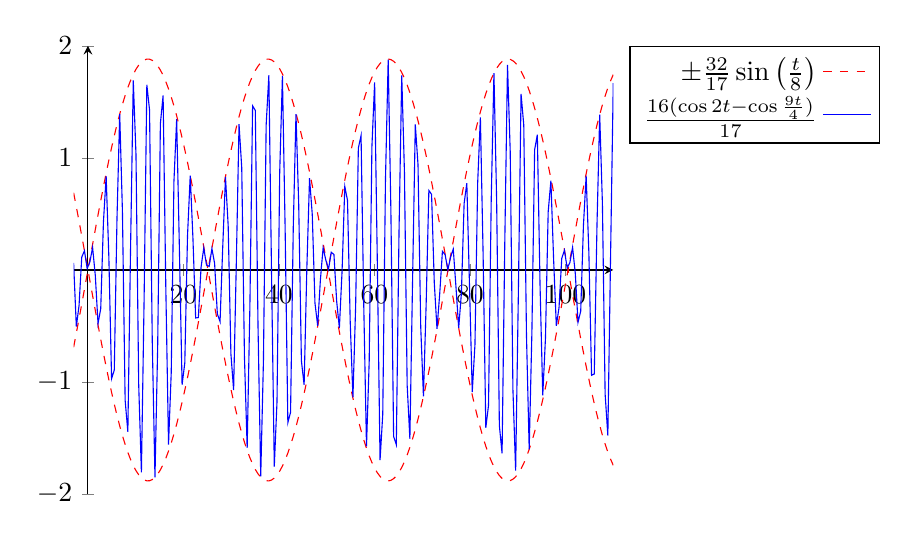
\begin{tikzpicture}
      \begin{axis}[
        xmin=-3,xmax=110,
        ymin=-2,ymax=2,
        legend pos=outer north east,
        axis lines=center,
        trig format plots=rad,
        legend style={legend cell align=right,legend plot pos=right}]

      \addplot[dashed,color=red,domain=-3:110,samples=200,forget plot] {(32/17)*sin(x/8)};
      \addplot[dashed,color=red,domain=-3:110,samples=200] {-(32/17)*sin(x/8)};
      \addlegendentry{$\pm\frac{32}{17}\sin\left(\frac{t}{8}\right)$}
      \addplot[color=blue,domain=-3:110,samples=200] {16*(cos(2*x)-cos((9/4)*x))/17};
      \addlegendentry{$\frac{16(\cos 2t-\cos\frac{9t}{4})}{17}$}
      \end{axis}
  \end{tikzpicture}
\end{center}

For \textbf{b)} the roots of the characteristic equation $s^2+4=0$ are still $s=\pm 2i$. So homogenous solution $y_h$ is still:
\begin{equation*}
  y_h(t)=k_1\cos2t+k_2\sin2t
\end{equation*}

However, the particular solution of our complexified equation $y''+4y=e^{2it}$ is now of the following form:
\begin{align*}
  y_c(t)&=Ate^{2it}\\
  y_c'(t)&=Ae^{2it}(1+2it)\\
  y_c''(t)&=4Aie^{2it}-4Ate^{2it}\\
  &=4Aie^{2it}-4y_c\\
\end{align*}

Solving for $A$ we find:
\begin{align*}
  y_c''+4y_c&=4Aie^{2it}\\
  e^{2it}&=4Aie^{2it}\\
  1&=4Ai\\
  A&=\frac{1}{4i}=\frac{-i}{4}
\end{align*}

And so our particular solution $y_p$ is:
\begin{align*}
  y_p(t)&=\Re{y_c(t)}\\
  &=\Re{Ate^{\frac{9it}{4}}}\\
  &=\Re{-\frac{ite^{2it}}{4}}\\
  &=\Re{-\frac{it(\cos 2t+i\sin2t)}{4}}\\
  &=\frac{t\sin2t}{4}
\end{align*}

And so the general solution $y$ is given by:
\begin{equation*}
  y(t)=k_1\cos2t+k_2\sin2t+\frac{t\sin2t}{4}
\end{equation*}

Now we simply have to find $k_1$ and $k_2$ that satisfy the initial conditions. First we set $y(0)=0$:
\begin{align*}
  0&=y(0)\\
  &=k_1\cos0+k_2\sin0+\frac{0}{4}\\
  &=k_1+0+0\\
  0&=k_1
\end{align*}

Now we set $y'(0)=0$:
\begin{align*}
  y'(t)&=-2k_1\sin2t+2k_2\cos2t+\frac{t\cos2t}{2}+\frac{\sin2t}{4}\\
  0=y'(0)&=-2k_1\sin0+2k_2\cos0+\frac{0}{2}+\frac{\sin0}{4}\\
  &=0+2k_2+0+0\\
 0&=k_2
\end{align*}

So the solution to the IVP is simply:
\begin{equation*}
  y_0(t)=\frac{t\sin2t}{4}
\end{equation*}

This gives us the following graph:
\begin{center}
  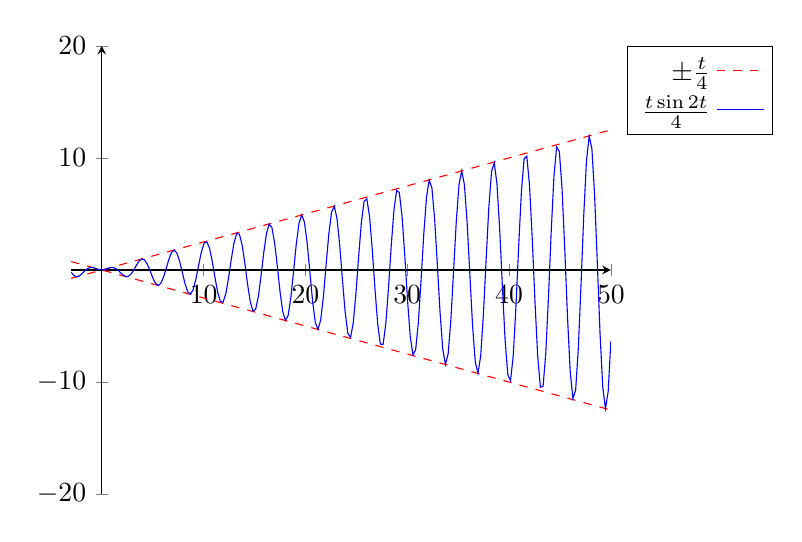
\begin{tikzpicture}
      \begin{axis}[
        xmin=-3,xmax=50,
        ymin=-20,ymax=20,
        legend pos=outer north east,
        axis lines=center,
        trig format plots=rad,
        legend style={legend cell align=right,legend plot pos=right}]

      \addplot[dashed,color=red,domain=-3:50,samples=200,forget plot] {x/4};
      \addplot[dashed,color=red,domain=-3:50,samples=200] {-x/4};
      \addlegendentry{$\pm\frac{t}{4}$}
      \addplot[color=blue,domain=-3:50,samples=200] {x*sin(2*x)/4};
      \addlegendentry{$\frac{t\sin2t}{4}$}
      \end{axis}
  \end{tikzpicture}
\end{center}

\section*{Problem 5}
\noindent\textbf{Problem:} Find and classify all the equilibria of the following system:
$$\begin{cases}
  x'=x(-x-3y+150)=-x^2-3xy+150x\\
  y'=y(-2x-y+100)=-2xy-y^2+100y
\end{cases}$$

\noindent\textbf{Solution:} By inspection, we note that this system has 4 equilibria:
\begin{enumerate}[label=\alph*)]
  \item $\vec p_1=(0,0)$
  \item $\vec p_2=(0,100)$
  \item $\vec p_3=(150,0)$
  \item $\vec p_4=(30,40)$
\end{enumerate}

Where the last equilibria is found by solving $\begin{cases}
  -x-3y+150\\
  -2x-y+100
\end{cases}$ To classify them via \textbf{linearization}, we must first compute the Jacobian of the system:
\begin{equation*}
  J\vec F=\begin{bmatrix}
    \der[x'][x] & \der[x'][y]\\
    \der[y'][x] & \der[y'][y]
  \end{bmatrix}=\begin{bmatrix}
    -2x-3y+150 & -3x\\
    -2y & -2x-2y+100
  \end{bmatrix}
\end{equation*}

Now, applying the Jacobian to each equilibrium, we find:
\begin{enumerate}[label=\alph*)]
  \item $J\vec F(0,0)=\begin{bmatrix}
    150 & 0\\
    0 & 100
  \end{bmatrix}$ Both eigenvalues $\lambda_1=150$ and $\lambda_2=100$ are positive, thus $\vec p_1$ is a source.
  \item $J\vec F(0,100)=\begin{bmatrix}
    -150 & 0\\
    -200 & -100
  \end{bmatrix}$ Both eigenvalues $\lambda_1=-150$ and $\lambda_2=-100$ are negative, thus $\vec p_2$ is a sink.
  \item $J\vec F(150,0)=\begin{bmatrix}
    -150 & -450\\
    0 & -200
  \end{bmatrix}$ Both eigenvalues $\lambda_1=-150$ and $\lambda_2=-200$ are negative, thus $\vec p_3$ is a sink.
  \item $J\vec F(30,40)=\begin{bmatrix}
    -30 & -90\\
    -80 & -40
  \end{bmatrix}$ The eigenvalues are roots of the equation $(\lambda+30)(\lambda+40)-90\cdot80$ which are $\lambda_1=-120$ and $\lambda=50$. This means $\vec p_4$ is a saddle.
\end{enumerate}

\section*{Problem 6}
\noindent\textbf{Problem:} Sketch the $x$-nullcline and $y$-nullcline of the system in problem 5. Then sketch its phase portrait.
\bigskip

\noindent\textbf{Solution:} The $x$-nullcines are:
\begin{equation*}
  x=0,\quad y=-\frac{x}{3}+50
\end{equation*}

And the $y$-nullcines are:
\begin{equation*}
  y=0,\quad y=-2x+100
\end{equation*}

Graphing the $x$-nullclines in red, the $y$-nullclines in blue, and drawing in some solutions, we arrive at:
\begin{center}
  \begin{tikzpicture}
      \begin{axis}[
        xmin=-30,xmax=180,
        ymin=-30,ymax=150,
        legend pos=outer north east,
        axis lines=center,
        trig format plots=rad,
        legend style={legend cell align=right,legend plot pos=right}]
      \addplot [color=red] coordinates {(0,-30) (0,150)};
      \addlegendentry{$x=0$}
      \addplot[color=red,domain=-30:180,samples=100] {-x/3+50};
      \addlegendentry{$y=-\frac{x}{3}+50$}
      \addplot[color=blue,domain=-30:180,samples=100] {0};
      \addlegendentry{$y=0$}
      \addplot[color=blue,domain=-30:180,samples=100] {-2*x+100};
      \addlegendentry{$y=-2x+100$}
      \end{axis}
  \end{tikzpicture}
\end{center}

\section*{Problem 7}
\noindent\textbf{Problem:} Find and classify all the equilibria of the following system:
$$\begin{cases}
  x'=x(2-x-y)=2x-x^2-xy\\
  y'=y(y-x^2)=y^2-x^2y
\end{cases}$$

\noindent\textbf{Solution:} By inspection, we note that this system has 4 equilibria:
\begin{enumerate}[label=\alph*)]
  \item $\vec p_1=(0,0)$
  \item $\vec p_2=(2,0)$
  \item $\vec p_3=(-2,4)$
  \item $\vec p_4=(1,1)$
\end{enumerate}

Where the last two equilibria are found by solving $\begin{cases}
  2-x-y\\
  y-x^2
\end{cases}$. The Jacobian of the system is given by:
\begin{equation*}
  J\vec F=\begin{bmatrix}
    \der[x'][x] & \der[x'][y]\\
    \der[y'][x] & \der[y'][y]
  \end{bmatrix}=\begin{bmatrix}
    2-2x-y & -x\\
    -2xy & 2y-x^2
  \end{bmatrix}
\end{equation*}

Now, applying the Jacobian to each equilibrium, we find:
\begin{enumerate}[label=\alph*)]
  \item $J\vec F(0,0)=\begin{bmatrix}
    2 & 0\\
    0 & 0
  \end{bmatrix}$ This matrix lies on the point $(2,0)$ in the trace-determinant plane and thus $\vec p_1$ is a degenerate equilibria with lines of parallel sources around it. 
  \item $J\vec F(2,0)=\begin{bmatrix}
    -2 & -2\\
    0 & -4
  \end{bmatrix}$ Both eigenvalues $\lambda_1=-2$ and $\lambda_2=-4$ are negative, thus $\vec p_2$ is a sink.
  \item $J\vec F(-2,4)=\begin{bmatrix}
    2 & 2\\
    16 & 4
  \end{bmatrix}$ This matrix lies on the point $(6,-24)$ in the trace-determinant plane and thus $\vec p_3$ is a saddle. 
  \item $J\vec F(1,1)=\begin{bmatrix}
    -1 & -1\\
    -2 & 1
  \end{bmatrix}$ This matrix lies on the point $(0,-3)$ in the trace-determinant plane and thus $\vec p_4$ is a saddle.
\end{enumerate}

\section*{Problem 8}
\noindent\textbf{Problem:} Sketch the $x$-nullcline and $y$-nullcline of the system in problem 7. Then sketch its phase portrait.
\bigskip

\noindent\textbf{Solution:} The $x$-nullcines are:
\begin{equation*}
  x=0,\quad y=2-x
\end{equation*}

And the $y$-nullcines are:
\begin{equation*}
  y=0,\quad y=x^2
\end{equation*}

Graphing the $x$-nullclines in red, the $y$-nullclines in blue, and drawing in some solutions, we arrive at:
\begin{center}
  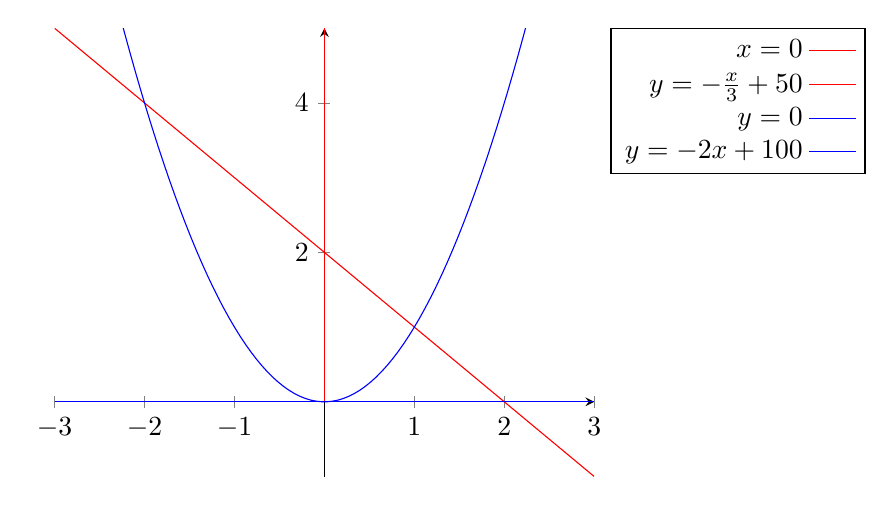
\begin{tikzpicture}
      \begin{axis}[
        xmin=-3,xmax=3,
        ymin=-1,ymax=5,
        legend pos=outer north east,
        axis lines=center,
        trig format plots=rad,
        legend style={legend cell align=right,legend plot pos=right}]
      \addplot [color=red] coordinates {(0,0) (0,5)};
      \addlegendentry{$x=0$}
      \addplot[color=red,domain=-3:3,samples=100] {2-x};
      \addlegendentry{$y=-\frac{x}{3}+50$}
      \addplot[color=blue,domain=-3:3,samples=100] {0};
      \addlegendentry{$y=0$}
      \addplot[color=blue,domain=-3:3,samples=100] {x^2};
      \addlegendentry{$y=-2x+100$}
      \end{axis}
  \end{tikzpicture}
\end{center}

\end{document}